\lecture{2010-01-20 Teil 2}
% Führe das Beispiel aus der letzten Vorlesung nahtlos fort.
\noindent $D=\mathbb{R}\setminus \{0\}$, $f(0)$ wird stetig ergänzt
\begin{proposition}\label{prop:equiv_zero}
  $\forall \nu$ gilt: $f^{(\nu)}(0) = 0$, damit $p(x) = 0 \text{ zu } x_0 = 0$
\end{proposition}

\begin{center}
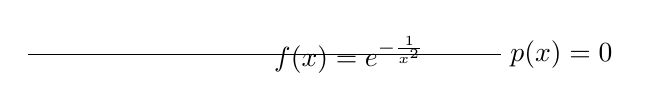
\begin{tikzpicture}
  \draw[domain=-3:3] plot [id=taylor_fail, samples=500] function {(2.71)**(-1/(x**2))} node [right] {$f(x)=e^{-\frac{1}{x^2}}$};
  \draw (-3,0) -- (3,0) node [right] {$p(x)=0$};
\end{tikzpicture}
\end{center}

\begin{proof}
  \begin{itemize}
    \item Induktionsvoraussetzung, $\nu = 1$
      \[ f'(x) = \euler^{-\frac{1}{x^2}}\cdot \frac{\diff}{\diff x}\left(-\frac{1}{x^2}\right) = \frac{2}{x^3}\cdot f(x) \]
      $f'(0)$ stetig ergänzbar zu $0$, da $\ds\lim_{x \rightarrow 0} f'(x) = 0$
    \item Induktionsschritt, $\nu = n + 1$\\
      Annahme: $f^{(\nu)}(x) = q_\nu(x)\cdot f(x)$ mit $\nu=1\ldots n$, $q_\nu(x)$ rationale Funktion
      \[
        f^{(n+1)}(x) = \left(\frac{\diff}{\diff x} q_n(x)\right)\cdot f(x) + \frac{2}{x^3} \cdot q_n(x) \cdot f(x)= q_{n+1}(x) \cdot f(x)
      \]
  \end{itemize}
  Ergebnis: $f^{(\nu)}(x) = q_\nu(x)\cdot f(x)$, $q_\nu$ rationale Funktion\\
  Verhalten in $x_0 = 0$:
  \begin{align*}
    \lim_{x\rightarrow \infty} \frac{\euler^x}{x^n} & = \infty & \forall n \in \mathbb{N}\\
    \lim_{x\rightarrow \infty} \frac{x^n}{\euler^x} & = 0 & \forall n \in \mathbb{N}\\
    \lim_{x\rightarrow 0} \frac{\euler^{-\frac{1}{x^2}}}{x^n} & = 0 & \leadsto f^{(n)}(0) = 0
  \end{align*}
  $\leadsto$ Behauptung \ref{prop:equiv_zero}: Taylorreihe $f \equiv 0 \neq \euler^{-\frac{1}{x^2}}$
\end{proof}

%\noindent offen: Konvergenz Taylorreihe zu $f(x)$\\
% Wieso offen? -LH
\noindent Die Taylorformel enthält das Restglied $R_\nu(x)$. Bildet die Folge der Restglieder $(R_\nu(x))_{\nu \in \mathbb{N}}$ eine Nullfolge, so konvergiert die Taylorreihe (als Grenzwert der Taylorpolynome) gegen $f(x)$.

\begin{note}Für $f(x) = \euler^{-\frac{1}{x^2}}$ bilden die Folgenglieder $R_\nu(x)$ keine Nullfolge.\end{note}

\todo[inline]{Anmerkung Landausymbole}
%\begin{note}
%Zu den Landausymbolen:\\
%Wir verstehen unter:
%\begin{itemize}
%
%   \item $R_{n+1}(x) = o(x)$ den Grenzwert für $x\to 0$:
%
%\end{itemize}
% TODO: Fertig machen
%\end{note}
